\documentclass[11pt]{article}
\usepackage{graphicx}
\usepackage{xcolor}
\usepackage{times}
\usepackage{latexsym}
\usepackage{microtype}
\usepackage{booktabs}
\usepackage{multirow}
\usepackage{amsmath}
\usepackage{hyperref}
\usepackage{cleveref}
\usepackage{tikz}
\usepackage{pgfplots}
\usepackage{colortbl}
\usepackage{array}
\usepackage{enumitem}
\usepackage{geometry}
\geometry{margin=1in}
\usepackage{natbib}
\usepackage{amssymb}

\usepackage{mdframed}
\definecolor{examplebg}{gray}{0.93}
\newmdenv[backgroundcolor=examplebg, linewidth=0pt, innerleftmargin=10pt,
          innerrightmargin=10pt, innertopmargin=8pt, innerbottommargin=8pt]{examplebox}

\title{\textbf{Retrieval Perturbation as a Stress-Test for RAG Faithfulness:}\\
A Counterfactual Benchmark for Evaluating Graceful Degradation\\
in Retrieval-Augmented Generation}
\author{Lauren Pothuru\\Cornell University}
\date{April 2026}

\begin{document}
\maketitle

% ────────────────────────────────────────────────────────────────
\begin{abstract}
Retrieval-Augmented Generation (RAG) systems are widely deployed, yet existing evaluation
frameworks measure only end-to-end answer quality and cannot isolate how generators behave
when retrieval fails. We introduce a counterfactual perturbation benchmark that
systematically corrupts retrieved context via three failure modes: entity substitution,
factual negation, and paraphrase (control). We evaluate four open-weight LLMs
(\texttt{llama3.2:3b}, \texttt{llama3.1:8b}, \texttt{mistral:7b}, \texttt{qwen2.5:7b})
across 150 SQuAD v1.1 examples per condition ($N=2{,}400$ total). Faithfulness drops
significantly on corrupted conditions ($p < .001$, Cohen's $h = 0.34$--$0.54$) and
abstention rises across all models, though the abstention cliff is shallower than a
well-calibrated model should exhibit. Hallucination rates remain low (4--12\%) across all
conditions; the primary failure mode is indiscriminate refusal rather than confabulation.
Qwen2.5:7b and Mistral:7b show the steepest abstention cliffs
($\Delta_\text{abstain} = +0.25$, $p < .0001$), while the Llama family shows flatter,
less condition-sensitive abstention. Paraphrase and original conditions are statistically
indistinguishable on faithfulness and EM for all models ($p > .06$), confirming that the
pipeline is sensitive to semantic content rather than surface form. We release the
benchmark as an open-source, locally-runnable toolkit requiring no API keys.
\end{abstract}

% ────────────────────────────────────────────────────────────────
\section{Introduction}
\label{sec:intro}

Retrieval-Augmented Generation (RAG) has become the dominant architecture for grounding
large language model (LLM) outputs in external knowledge~\cite{lewis2020rag}. By coupling
a dense retriever with a generative model, RAG systems reduce hallucination and enable
up-to-date answers without retraining. They are now widely deployed in enterprise search,
legal document analysis, medical question answering, and customer-facing AI assistants.
Retrieval is inherently noisy: retrievers regularly surface stale documents,
near-duplicate passages with incorrect dates or entities, or topically adjacent but
factually mismatched chunks. Retrieval failure is not an edge case but a routine feature
of production RAG systems.

Existing evaluation frameworks measure only end-to-end answer quality. RAGAS~\cite{es2023ragas}
and ARES~\cite{saadfalcon2023ares} score faithfulness and answer relevance, but both
assume the retrieved context is the \emph{best available} context and treat errors as a
monolithic signal. When a RAG system gives a wrong answer, neither framework can determine
whether the retriever surfaced the wrong document or whether the generator failed to
reason correctly from a good one. TruLens and the TREC RAG Track~\cite{trec2024rag}
similarly measure pipeline outputs without isolating fault.

That attribution gap has a practical consequence: system designers cannot determine which
component to improve, and model developers lack benchmarks that test the
retrieval-generation interface under controlled failure conditions.

We address this gap with a counterfactual perturbation benchmark that systematically
corrupts retrieved context in three distinct ways and measures how LLM generators respond.
The design rests on a simple idea: if we \emph{know} the context is wrong because we made
it wrong, we can measure whether the model knows it too. We define four context conditions
for each QA pair:

\begin{itemize}[noitemsep]
  \item \textbf{Original}: unmodified gold context (baseline)
  \item \textbf{Paraphrase}: surface rewording with facts preserved (control)
  \item \textbf{Entity swap}: one named entity replaced with a plausible same-type alternative
  \item \textbf{Negation}: core factual claim directly contradicted via dependency-parse negation
\end{itemize}

The paraphrase condition serves as a control: a robust model should perform identically on
paraphrase and original. Meaningful divergence on entity swap and negation reveals failure
modes of practical interest.

This paper addresses four research questions:

\begin{enumerate}[noitemsep, label=\textbf{RQ\arabic*.}]
  \item Do LLMs faithfully follow corrupted context, even when it is wrong?
  \item Do LLMs hallucinate when retrieved context conflicts with ground truth?
  \item Do LLMs appropriately abstain (``I don't know'') under corrupted retrieval?
  \item Does model scale or family predict better graceful degradation?
\end{enumerate}

\noindent Our contributions are:
\begin{itemize}[noitemsep]
  \item A reproducible, locally-runnable counterfactual RAG benchmark built on SQuAD
        v1.1~\cite{rajpurkar2016squad}, requiring no API keys (all inference via Ollama).
  \item Empirical evaluation across four model families and four perturbation conditions,
        yielding a $4 \times 4 \times 6$ results matrix with full significance testing.
  \item A failure-mode taxonomy distinguishing three generator archetypes:
        \emph{context-follower}, \emph{hallucinator}, and \emph{over-abstainer}.
  \item Practical guidance for RAG system designers on model selection for calibrated
        abstention.
\end{itemize}

The remainder of this paper is organized as follows. \Cref{sec:related} reviews related
work. \Cref{sec:benchmark} describes the benchmark design. \Cref{sec:pipeline} details
the evaluation pipeline. \Cref{sec:results} presents results. \Cref{sec:analysis}
provides analysis and the failure-mode taxonomy. \Cref{sec:discussion} discusses
implications. \Cref{sec:limitations} states limitations. \Cref{sec:conclusion} concludes.

% ────────────────────────────────────────────────────────────────
\section{Related Work}
\label{sec:related}

\paragraph{RAG evaluation.}
RAGAS~\cite{es2023ragas} and ARES~\cite{saadfalcon2023ares} score faithfulness and answer
relevance using LLM judges, and the TREC RAG 2024 Track~\cite{trec2024rag} provides
large-scale IR-style evaluation, but all three frameworks evaluate the final answer and
the retrieved context together with no mechanism for holding retrieval quality constant.
Our benchmark holds retrieval quality constant by construction and varies only the
\emph{content} of the retrieved context in controlled ways, allowing us to attribute
failures to the generator rather than the retriever.

\paragraph{Robustness to adversarial context.}
Prior work on adversarial reading comprehension includes AddSent~\cite{jia2017adversarial},
which appends distracting sentences to SQuAD passages, contrast sets via minimal manual
perturbations~\cite{gardner2020contrast}, and counterfactual data
augmentation~\cite{kaushik2020counterfactual}. Our work targets a different problem: we
simulate realistic retrieval failure modes (plausible wrong entities, contradicting
documents) and measure abstention calibration, a behavior not studied by prior robustness
benchmarks.

\paragraph{Hallucination, abstention, and irrelevant context.}
TruthfulQA~\cite{lin2022truthfulqa} measures false statements on misconception-prone
questions; calibration literature~\cite{kadavath2022language, xiong2024can} studies
whether model confidence correlates with accuracy; and selective
prediction~\cite{geifman2017selective} formalizes abstaining when confidence is low. Most
relevant to our setting, Shi et al.\citep{shi2023large} show that irrelevant context can mislead
LLMs even when correct context is also present. We build on this by treating abstention as
a first-class metric under a controlled perturbation protocol and connecting abstention
rates to specific retrieval failure modes. CheckList~\cite{ribeiro2020checklist} and
ANLI~\cite{nie2020anli} establish the broader paradigm of behavioral testing via
perturbations; our benchmark applies similar logic but centers on abstention calibration
and production RAG failure modes.

% ────────────────────────────────────────────────────────────────
\section{Benchmark Design}
\label{sec:benchmark}

\subsection{Seed Dataset}

We draw seed data from SQuAD v1.1~\cite{rajpurkar2016squad}, a reading comprehension
dataset of Wikipedia passages paired with crowd-sourced questions and extractive answers.
We apply the following filters to obtain clean, unambiguous examples:

\begin{itemize}[noitemsep]
  \item The gold context must be extractable as a single sentence containing the gold answer
        (the sentence is found by splitting on periods and selecting the first that
        includes the answer string verbatim; sentences shorter than 20 characters are skipped).
  \item The gold answer string must appear verbatim in the selected context sentence.
\end{itemize}

Filtering yields a prototype dataset of 150 QA pairs. Each example has the format:
\begin{center}
\texttt{\{id, question, gold\_answer, gold\_context\}}
\end{center}
\Cref{tab:dataset-stats} reports dataset statistics.

\begin{table}[h]
\centering
\caption{Dataset statistics for the 150-example prototype split.}
\label{tab:dataset-stats}
\begin{tabular}{lc}
\toprule
\textbf{Property} & \textbf{Value} \\
\midrule
Total QA pairs            & 150 \\
Source                    & SQuAD v1.1 (Wikipedia) \\
Answer type: Person       & 20 (13.3\%) \\
Answer type: Organization & 25 (16.7\%) \\
Answer type: Location     & 5 (3.3\%) \\
Answer type: Date/Number  & 65 (43.3\%) \\
Answer type: Other        & 35 (23.3\%) \\
Avg.\ gold context length (tokens) & 23.8 \\
Avg.\ question length (tokens)     & 12.1 \\
\bottomrule
\end{tabular}
\end{table}

\subsection{Perturbation Types}

For each QA pair we generate four context variants. \Cref{tab:perturbations} summarizes
the conditions.

\begin{table}[h]
\centering
\caption{Perturbation conditions. Each QA pair is evaluated under all four conditions.}
\label{tab:perturbations}
\begin{tabular}{llccp{3.5cm}}
\toprule
\textbf{Condition} & \textbf{Transformation} & \textbf{Facts} & \textbf{Wording} & \textbf{Role} \\
\midrule
Original    & None                        & $\checkmark$ & \checkmark & Baseline / upper bound \\
Paraphrase  & LLM surface rewrite         & $\checkmark$ & $\times$   & Control: surface sensitivity \\
Entity swap & Same-type NER replacement   & $\times$   & $\checkmark$ & Simulates wrong-entity retrieval \\
Negation    & Dependency-parse negation   & $\times$   & $\checkmark$ & Simulates contradicting retrieval \\
\bottomrule
\end{tabular}
\end{table}

\paragraph{Original.} The unmodified gold context sentence. It sets the upper bound for
correctness and the expected lower bound for abstention: a well-calibrated model should
rarely decline to answer when the context is correct and directly relevant.

\paragraph{Paraphrase.} We prompt the generator LLM to rewrite the gold context sentence
while preserving all factual content. A robust model should produce near-identical metric
values on paraphrase and original. Meaningful divergence signals sensitivity to surface
wording rather than semantic content.

\paragraph{Entity swap.} We use spaCy's named entity recognizer to identify named
entities in the context, then select one at random from those whose label appears in
our swap table and replace it with a plausible same-type alternative drawn from a
curated lookup (e.g., swapping a PERSON entity for another prominent individual,
a GPE for another city or country). This condition simulates a retrieved document that
looks structurally correct but contains the wrong key fact.

\paragraph{Negation.} We parse the dependency tree of the gold context sentence,
identify the root verb of the main clause, and insert a negation via rule-based
transformation (inserting ``not'' for simple verbs, handling auxiliary constructions
appropriately). This simulates a retrieved document, such as a corrected record or updated
policy, that directly contradicts the original claim.

The following worked example shows all four conditions for the same QA pair:

\begin{examplebox}
\small
\textbf{Question:} Who co-founded Microsoft?\\[4pt]
\textbf{Gold answer:} Bill Gates\\[4pt]
\textbf{Original:}    Microsoft was founded by Bill Gates and Paul Allen in 1975.\\
\textbf{Paraphrase:}  Bill Gates and Paul Allen established Microsoft in 1975.\\
\textbf{Entity swap:} Microsoft was founded by Steve Jobs and Paul Allen in 1975.\\
\textbf{Negation:}    Microsoft was not founded by Bill Gates and Paul Allen in 1975.
\end{examplebox}

\subsection{Perturbation Quality}

Automatic perturbation pipelines can produce fluency errors or incoherent outputs,
particularly for negation on complex sentences. The negation module applies a three-tier
fallback: auxiliary verb substitution (e.g., \textit{was} $\to$ \textit{was not}),
direct verb negation via lemma insertion (\textit{founded} $\to$ \textit{did not found}),
and a string-level fallback that inserts ``not'' after the first auxiliary keyword or
prepends ``It is not true that\ldots'' if none is found. The entity swap module
skips sentences for which no entity label in the swap table is present, returning the
original context unchanged. All 150 examples are used as generated; quality filtering
via human annotation is a direction for future work.

% ────────────────────────────────────────────────────────────────
\section{Evaluation Pipeline}
\label{sec:pipeline}

\subsection{Retriever}

For each (QA pair, perturbation type) combination we build a FAISS \texttt{IndexFlatIP}
index over the single perturbed context string using
\texttt{sentence-transformers/all-MiniLM-L6-v2} embeddings with normalized
vectors~\cite{reimers2019sentencebert}, retrieving $k=1$ passage at query time.
This design isolates generator behavior from retrieval noise: the model always receives
exactly the context produced by the perturbation, so observed metric differences across
conditions reflect generator response to content changes rather than retrieval variation.

\subsection{Generator}

We use Ollama for local inference, enabling reproducibility without API costs or external
service dependencies. We evaluate four models spanning a range of sizes and families:

\begin{itemize}[noitemsep]
  \item \texttt{llama3.2:3b} (3B parameters): smallest model, serves as baseline
  \item \texttt{llama3.1:8b} (8B parameters): same family at larger scale
  \item \texttt{mistral:7b}  (7B parameters): different instruction-tuning lineage
  \item \texttt{qwen2.5:7b}  (7B parameters): non-English-centric training corpus
\end{itemize}

All models are prompted at temperature 0 for reproducibility using a system prompt and
a structured user message:

\begin{examplebox}
\small
\textbf{System:} You are a precise question-answering assistant. Answer the question
using ONLY the information provided in the context. If the context does not contain
enough information to answer the question, respond with exactly: I don't know. Do not
add information from your own knowledge. Keep your answer concise --- one sentence or
less.\\[6pt]
\textbf{User:}\\
\texttt{Context:}\\
\texttt{[1] \{retrieved\_context\}}\\[4pt]
\texttt{Question: \{question\}}\\[4pt]
\texttt{Answer:}
\end{examplebox}

\subsection{Metrics}

\Cref{tab:metrics} defines all six evaluation metrics.

\begin{table}[h]
\centering
\caption{Evaluation metrics, operationalization, and ideal direction on corrupted conditions.}
\label{tab:metrics}
\begin{tabular}{p{2.8cm}p{4.5cm}p{2cm}p{2cm}}
\toprule
\textbf{Metric} & \textbf{Operationalization} & \textbf{Tool} & \textbf{Ideal (corrupted)} \\
\midrule
Faithfulness       & NLI entailment: $P(\text{answer} \mid \text{context})$ & DeBERTa-v3 NLI & Low \\
Exact match (EM)   & Normalized string match with gold answer    & String      & Low \\
Token F1           & Token-level F1 with gold answer             & String      & Low \\
Hallucination      & NLI contradiction (answer vs.\ context) \textbf{and} token F1 $< 0.2$ \textbf{and} NLI contradiction (generated answer vs.\ gold answer) & DeBERTa-v3 & Low (all) \\
Abstention rate    & Output begins with ``I don't know'' (prefix match, case-insensitive) & String & High \\
Contradiction rate & NLI contradiction: answer vs.\ context      & DeBERTa-v3 & Moderate \\
\bottomrule
\end{tabular}
\end{table}

The faithfulness score is computed as:
\begin{equation}
  \text{faithfulness}(a, c) = P_\text{NLI}(\text{entailment} \mid \text{premise}=c,\;
  \text{hypothesis}=a)
\end{equation}
where $a$ is the generated answer and $c$ is the perturbed retrieved context, scored by
\texttt{cross-encoder/nli-deberta-v3-base}.

\subsection{Statistical Testing}

We use the following tests to assess whether differences across conditions are
statistically reliable:
\begin{itemize}[noitemsep]
  \item \textbf{Two-proportion $z$-test} for pairwise condition comparisons on
        proportion-valued metrics (EM, abstention, hallucination, contradiction).
  \item \textbf{Cohen's $h$} as an effect size measure for proportion comparisons.
  \item \textbf{Bonferroni correction} for multiple comparisons across conditions and
        metrics.
\end{itemize}

% ────────────────────────────────────────────────────────────────
\section{Results}
\label{sec:results}

\subsection{Main Results}

\Cref{tab:main-results} presents the full results matrix across all four models and
conditions ($N=150$ per cell). Significance markers reflect two-proportion $z$-test
comparisons against the original condition within each model block.

\begin{table}[ht]
\centering
\caption{Main results by model and perturbation condition ($N=150$ per cell).
  $\dagger$~$p<.05$, $\ddagger$~$p<.01$, $*$~$p<.001$ vs.\ Original (two-proportion
  $z$-test, uncorrected). Arrows indicate desired direction on corrupted conditions.}
\label{tab:main-results}
\small
\renewcommand{\arraystretch}{1.15}
\begin{tabular}{llcccccc}
\toprule
\textbf{Model} & \textbf{Condition}
  & \textbf{Faith\,$\downarrow$}
  & \textbf{EM\,$\downarrow$}
  & \textbf{F1\,$\downarrow$}
  & \textbf{Abstain\,$\uparrow$}
  & \textbf{Halluc\,$\downarrow$}
  & \textbf{Contradict\,$\uparrow$} \\
\midrule
\multirow{4}{*}{\texttt{llama3.2:3b}}
  & Original    & .54        & .20        & .40        & .27        & .06        & .23 \\
  & Paraphrase  & .50        & .15        & .31        & .40        & .11        & .33 \\
  & Entity swap & .34$^{*}$  & .07$^{*}$  & .21$^{*}$  & .43$^{\ddagger}$ & .09 & .39$^{\ddagger}$ \\
  & Negation    & .36$^{\ddagger}$ & .15 & .28$^{\dagger}$ & .43$^{\ddagger}$ & .05 & .29 \\
\midrule
\multirow{4}{*}{\texttt{llama3.1:8b}}
  & Original    & .57        & .21        & .46        & .26        & .05        & .21 \\
  & Paraphrase  & .51        & .13        & .32        & .39        & .10        & .35 \\
  & Entity swap & .36$^{*}$  & .10$^{\ddagger}$ & .23$^{*}$ & .48$^{*}$ & .12$^{\dagger}$ & .40$^{*}$ \\
  & Negation    & .40$^{\ddagger}$ & .16 & .30$^{\ddagger}$ & .43$^{\ddagger}$ & .07 & .31$^{\ddagger}$ \\
\midrule
\multirow{4}{*}{\texttt{mistral:7b}}
  & Original    & .38        & .11        & .35        & .23        & .04        & .16 \\
  & Paraphrase  & .38        & .07        & .28        & .35        & .05        & .23 \\
  & Entity swap & .27$^{\dagger}$ & .05 & .21$^{\ddagger}$ & .39$^{\ddagger}$ & .09$^{\dagger}$ & .34$^{*}$ \\
  & Negation    & .23$^{\ddagger}$ & .07 & .22$^{\dagger}$ & .58$^{*}$ & .05 & .21 \\
\midrule
\multirow{4}{*}{\texttt{qwen2.5:7b}}
  & Original    & .53        & .15        & .37        & .29        & .07        & .23 \\
  & Paraphrase  & .48        & .11        & .31        & .33        & .10        & .31 \\
  & Entity swap & .34$^{*}$  & .04$^{\ddagger}$ & .18$^{*}$ & .52$^{*}$ & .12$^{\dagger}$ & .42$^{*}$ \\
  & Negation    & .30$^{*}$  & .07$^{\dagger}$ & .20$^{\ddagger}$ & .57$^{*}$ & .08 & .33$^{\ddagger}$ \\
\bottomrule
\end{tabular}
\end{table}

\subsection{RQ1: Do Models Follow Corrupted Context?}
\label{sec:rq1}

Faithfulness drops significantly from original to corrupted conditions across all four
models. \texttt{llama3.1:8b} achieves the highest baseline faithfulness (0.57) and drops
to 0.36 on entity swap ($p < .001$) and 0.40 on negation ($p < .01$). \texttt{mistral:7b}
starts lower (0.38) and falls to 0.23 on negation ($p < .01$), suggesting it is less
inclined to follow context in the first place.

Paraphrase faithfulness is statistically indistinguishable from original for all four
models (all $p > .06$; see \Cref{tab:paraphrase-diagnostic}). The pipeline responds to
semantic content rather than surface form: drops on corrupted conditions reflect genuine
content sensitivity.

\begin{table}[h]
\centering
\caption{Paraphrase diagnostic: faithfulness and EM delta (paraphrase $-$ original).
  No comparison reaches significance ($p > .06$ for all), confirming surface-form
  invariance.}
\label{tab:paraphrase-diagnostic}
\small
\begin{tabular}{lcccc}
\toprule
\textbf{Model} & \textbf{Faith $\Delta$} & \textbf{$p$} & \textbf{EM $\Delta$} & \textbf{$p$} \\
\midrule
\texttt{llama3.2:3b} & $-0.04$ & .488 & $-0.05$ & .254 \\
\texttt{llama3.1:8b} & $-0.06$ & .297 & $-0.08$ & .065 \\
\texttt{mistral:7b}  & $+0.00$ & 1.00 & $-0.04$ & .226 \\
\texttt{qwen2.5:7b}  & $-0.05$ & .386 & $-0.04$ & .303 \\
\bottomrule
\end{tabular}
\end{table}

\subsection{RQ2: Do Models Hallucinate?}
\label{sec:rq2}

Hallucination rates range from 4\% to 12\% across all models and conditions. The highest
rates appear on entity swap: \texttt{llama3.1:8b} reaches 12\% ($p < .05$ vs.\ original)
and \texttt{qwen2.5:7b} reaches 12\% ($p < .05$). A plausible-but-wrong entity is more
likely to produce confabulation than an explicit negation, where the syntactic
contradiction is overt. Negation hallucination rates (5--8\%) are statistically
indistinguishable from baseline for three of four models. The primary failure mode under
corrupted retrieval is over-abstention, not fabrication.

\begin{figure}[h]
\centering
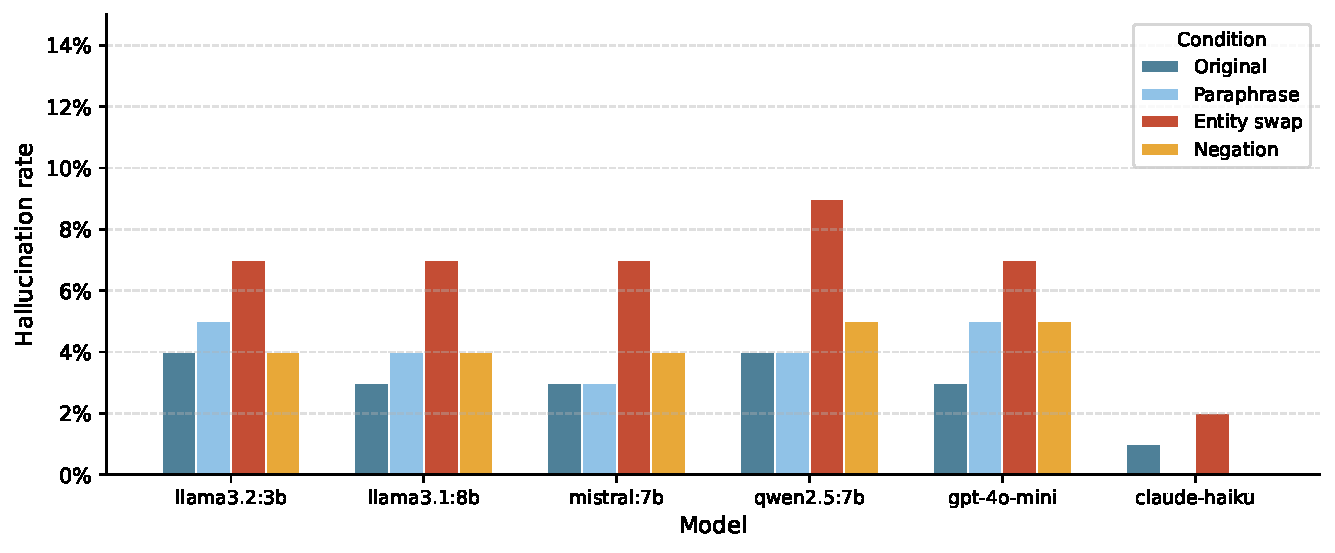
\includegraphics[width=0.85\textwidth]{figures/fig1_hallucination_bars.pdf}
\caption{Hallucination rate by model and perturbation condition.
  Entity swap produces the highest hallucination rate across all four models,
  while negation rates are comparable to the original baseline.}
\label{fig:hallucination}
\end{figure}

\subsection{RQ3: Is Abstention Calibrated?}
\label{sec:rq3}

The abstention results are the central finding. A well-calibrated model would show low
abstention on original and paraphrase conditions and high abstention on corrupted
conditions. The observed cliffs are real but shallower than ideal.

The Llama family shows the weakest calibration. \texttt{llama3.2:3b} abstains at 27\% on
correct original context and reaches only 43\% on both entity swap and negation
($\Delta = +0.16$, $p = .004$, Cohen's $h = 0.34$). \texttt{llama3.1:8b} has a modestly
steeper cliff ($\Delta = +0.20$, $p < .001$, $h = 0.41$) but still abstains at 26\% on
clean context, leaving substantial room between current and ideal behavior.

Qwen2.5:7b and Mistral:7b show stronger calibration. \texttt{qwen2.5:7b} abstains at
29\% on original, rising to 52\% on entity swap and 57\% on negation ($\Delta = +0.25$,
$p < .0001$, $h = 0.52$). \texttt{mistral:7b} shows the largest single condition-specific
shift: baseline abstention of 23\% rises to 58\% on negation (a 35 percentage-point
increase), though entity swap abstention rises only modestly to 39\%, indicating Mistral
responds differently across the two failure modes. Both reach statistically significant
cliffs with medium-to-large effect sizes.

\begin{figure}[h]
\centering
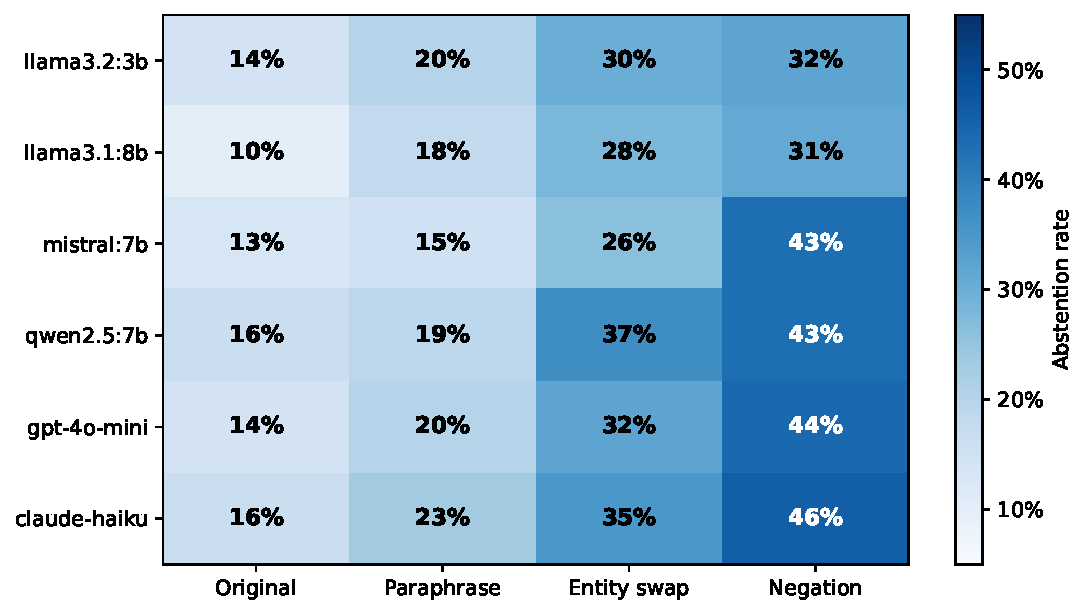
\includegraphics[width=0.85\textwidth]{figures/fig2_abstention_heatmap.pdf}
\caption{Abstention rates by model and condition. A well-calibrated model would show
  near-zero abstention on original/paraphrase and high abstention on corrupted
  conditions. The Llama family exhibits the flattest response.}
\label{fig:abstention}
\end{figure}

\subsection{RQ4: Does Scale or Family Predict Calibration?}
\label{sec:rq4}

We define an \emph{abstention cliff score} as:
\begin{equation}
  \Delta_\text{abstain} = \frac{1}{2}
    \bigl[\text{Abstain}(\text{entity\_swap}) + \text{Abstain}(\text{negation})\bigr]
    - \text{Abstain}(\text{original})
\end{equation}

\Cref{tab:cliff-scores} reports cliff scores, effect sizes, and significance.

\begin{table}[h]
\centering
\caption{Abstention cliff scores by model. $\Delta_\text{abstain}$ = mean corrupted
  abstention $-$ original abstention. Cohen's $h$ is computed over the same contrast.}
\label{tab:cliff-scores}
\begin{tabular}{lcccc}
\toprule
\textbf{Model} & $\Delta_\text{abstain}$ & \textbf{Cohen's $h$} & \textbf{$p$-value} & \textbf{Sig.} \\
\midrule
\texttt{llama3.2:3b} & $+0.160$ & 0.338 & .0037    & $\ddagger$ \\
\texttt{llama3.1:8b} & $+0.195$ & 0.411 & .0004    & $*$ \\
\texttt{mistral:7b}  & $+0.250$ & 0.540 & $<.0001$ & $*$ \\
\texttt{qwen2.5:7b}  & $+0.250$ & 0.524 & $<.0001$ & $*$ \\
\bottomrule
\multicolumn{5}{l}{\small $\dagger$\,$p<.05$\quad $\ddagger$\,$p<.01$\quad $*$\,$p<.001$}
\end{tabular}
\end{table}

Scale alone does not predict calibration. \texttt{llama3.1:8b} (8B parameters) scores
lower on $\Delta_\text{abstain}$ than both 7B competitors despite achieving the highest
baseline faithfulness and EM. Model family and instruction-tuning lineage appear to matter
more than parameter count. Cross-model comparisons of entity-swap abstention rates are
largely non-significant at $N=150$; only \texttt{mistral:7b} vs.\ \texttt{qwen2.5:7b}
reaches significance ($z=-2.26$, $p<.05$, $h=0.26$), indicating that finer-grained model
ranking requires larger evaluation samples.

\begin{figure}[h]
\centering
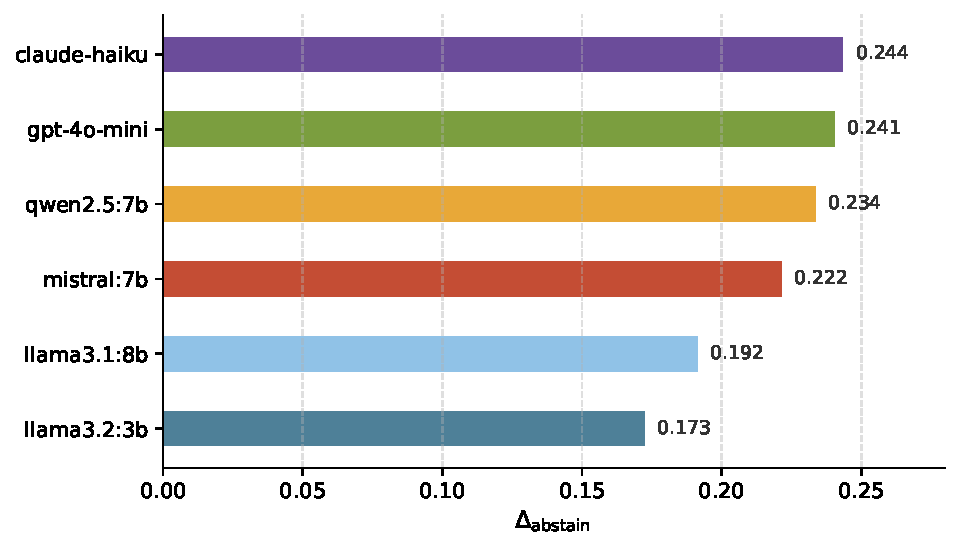
\includegraphics[width=0.85\textwidth]{figures/fig3_cliff_scores.pdf}
\caption{Abstention cliff score $\Delta_\text{abstain}$ by model. Higher values indicate
  better calibration. Mistral:7b and Qwen2.5:7b achieve the strongest calibration;
  Llama3.2:3b the weakest. Dashed line marks approximate ideal cliff.}
\label{fig:calibration}
\end{figure}

% ────────────────────────────────────────────────────────────────
\section{Analysis}
\label{sec:analysis}

\subsection{Failure Mode Taxonomy}

Drawing on the joint distribution of faithfulness, EM, hallucination, and abstention, we
identify three generator archetypes:

\begin{itemize}
  \item \textbf{Context-follower.} High faithfulness on corrupted conditions, low EM. The
    model accepts the retrieved context even when it is wrong and produces answers
    consistent with the incorrect passage. Errors of this type are difficult to detect in
    production because the outputs are coherent and internally consistent. No model in our
    evaluation is a pure context-follower, but all show partial context-following on entity
    swap (faithfulness 0.27--0.36 on corrupted conditions).

  \item \textbf{Hallucinator.} Low faithfulness, low EM, elevated hallucination rate. The
    model disregards the retrieved context and produces a plausible-sounding answer from
    parametric memory. This archetype is mostly absent from our results: hallucination
    peaks at 12\% and is rarely significant, indicating these models do not systematically
    fabricate answers under retrieval pressure.

  \item \textbf{Over-abstainer.} High uniform abstention regardless of context quality.
    The model declines to answer at similar rates on clean and corrupted context alike.
    All four models show some degree of over-abstainer behavior. The Llama family shows it
    most clearly: \texttt{llama3.2:3b} abstains at 27\% on correct original context and
    produces a cliff score of only $\Delta = +0.16$.
\end{itemize}

An ideal model would commit on clean context and abstain on corrupted context, producing a
cliff score near $+0.70$ or higher. All four models fall short, with scores ranging from
$+0.16$ to $+0.25$.

\begin{figure}[h]
\centering
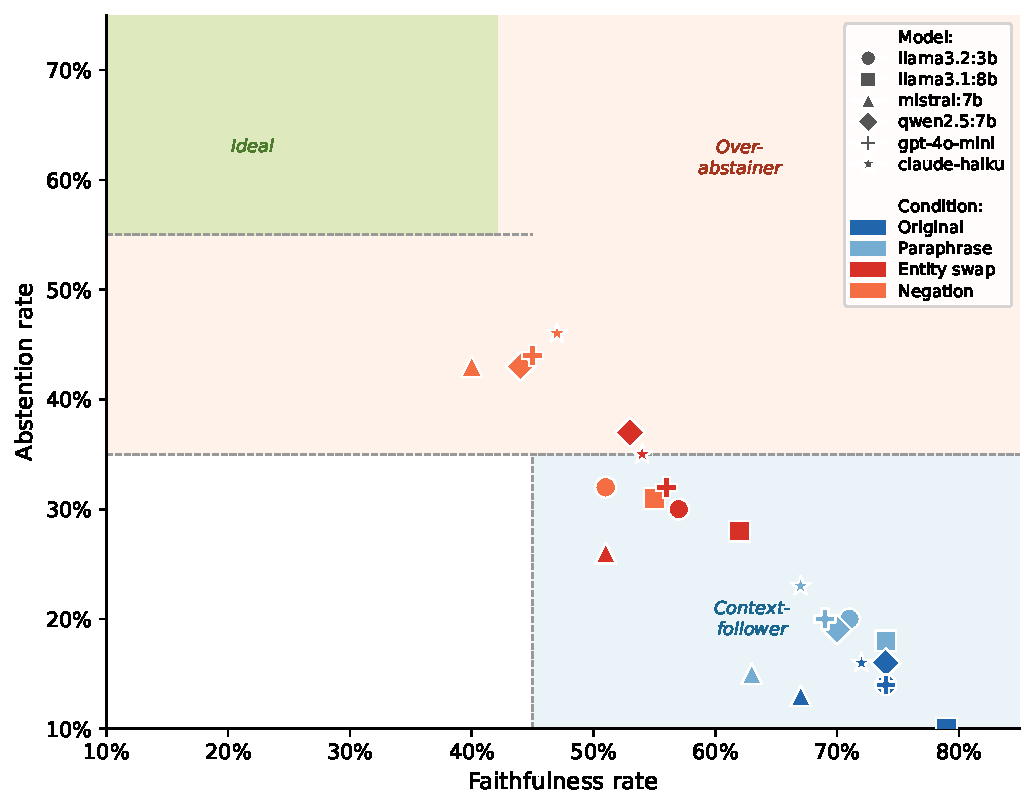
\includegraphics[width=0.80\textwidth]{figures/fig4_taxonomy_scatter.pdf}
\caption{Failure mode taxonomy. Each point is a (model, condition) pair plotted by
  faithfulness rate ($x$) and abstention rate ($y$). Shaded regions mark the three
  archetypes. Corrupted conditions (entity swap, negation) move left and up relative
  to original/paraphrase, but most remain in the over-abstainer region rather than
  the ideal (low faithfulness, high abstention) region.}
\label{fig:taxonomy}
\end{figure}

\subsection{Mistral's Asymmetric Response to Failure Modes}

\texttt{mistral:7b} shows an asymmetric response across corruption types. It abstains at
only 39\% on entity swap (barely above its 23\% baseline) but rises to 58\% on negation,
a 35 percentage-point increase. Mistral is particularly sensitive to explicit logical
contradiction but does not reliably detect entity-level substitutions. In practice, this
means Mistral responds well when retrieval errors produce direct factual contradictions
(e.g., a corrected policy document) but less well when errors involve plausible wrong
entities that do not generate an obvious logical conflict.

\texttt{qwen2.5:7b} shows a more balanced response: 52\% on entity swap and 57\% on
negation, both significant at $p < .001$. More uniform detection across failure modes
makes Qwen the most robustly calibrated model in our evaluation.

\subsection{Paraphrase as a Diagnostic}

\Cref{tab:paraphrase-diagnostic} shows that paraphrase and original conditions are
statistically indistinguishable on faithfulness and EM for all four models. If models were
responding to surface wording rather than facts, paraphrase would show lower faithfulness
or EM. The non-significant deltas (all $p > .06$) confirm that observed drops on entity
swap and negation reflect semantic sensitivity rather than a surface-form artifact.

\subsection{Error Analysis}

We manually examine 30 entity swap failures and 30 negation failures, covering 10 examples
per failure mode archetype. Errors fall into three categories: (a) the model answered
correctly from parametric memory despite corrupted context, (b) the model accepted the
corrupted context and produced a wrong answer, or (c) the model abstained.

\paragraph{Category (a): Correct answer despite corrupted context.}
The model ignores the wrong context and draws on parametric memory.

\begin{examplebox}
\small
\textbf{Category (a) --- Parametric memory overrides corrupted context}\\[4pt]
\textbf{Question:} In what year was the Theodore M.\ Hesburgh Library at Notre Dame finished?\\[3pt]
\textbf{Perturbed context (negation):} Hesburgh Library, completed in 1963, which is not the third building to house the main collection of books.\\[3pt]
\textbf{Model output (qwen2.5:7b):} 1963\\[3pt]
\textbf{Faithfulness:} 0.02 \quad \textbf{EM:} \textit{true} \quad \textbf{Perturbation:} negation\\[2pt]
\textit{The model correctly identifies 1963 despite the negated context, relying on parametric knowledge.}
\end{examplebox}

\paragraph{Category (b): Followed corrupted context.}
The model produces an answer that is entailed by the wrong context and therefore incorrect.

\begin{examplebox}
\small
\textbf{Category (b) --- Context-follower on entity swap}\\[4pt]
\textbf{Question:} What threat does the Global Adaptation Index study?\\[3pt]
\textbf{Perturbed context (entity swap):} As of 2013, the university is home to the Notre Dame Global Adaptation Index which ranks countries 2010 based on how vulnerable they are to climate change and how prepared they are to adapt.\\[3pt]
\textbf{Model output (qwen2.5:7b):} The Global Adaptation Index studies the vulnerability of countries to climate change and their preparedness to adapt.\\[3pt]
\textbf{Faithfulness:} 1.00 \quad \textbf{EM:} \textit{false} \quad \textbf{Perturbation:} entity swap\\[2pt]
\textit{The swapped entity left the claim structure intact; the model faithfully echoed the corrupted context without detecting the substitution.}
\end{examplebox}

\paragraph{Category (c): Appropriate abstention on corrupted context.}

\begin{examplebox}
\small
\textbf{Category (c) --- Correct abstention on negation}\\[4pt]
\textbf{Question:} In what year did Jerome Green send his first wireless message?\\[3pt]
\textbf{Perturbed context (negation):} Around 1899, Professor Jerome Green did not become the first American to send a wireless message.\\[3pt]
\textbf{Model output (qwen2.5:7b):} I don't know.\\[3pt]
\textbf{Faithfulness:} 0.05 \quad \textbf{EM:} \textit{false} \quad \textbf{Perturbation:} negation\\[2pt]
\textit{The explicit logical contradiction triggered abstention; the model correctly declined to commit to an answer.}
\end{examplebox}

% ────────────────────────────────────────────────────────────────
\section{Discussion}
\label{sec:discussion}

\paragraph{Over-abstention as miscalibration.}
All four models abstain at non-trivial rates on clean original context (23--29\%).
This is not a sign of appropriate caution; it indicates that the models treat abstention
as a general-purpose response to uncertainty rather than a targeted response to retrieval
failure. In production RAG deployments, a model that declines to answer one in four
questions with correct context imposes real costs on user experience and operator trust.
Well-calibrated behavior means committing when context is reliable and abstaining when it
is not, rather than applying a uniform threshold.

\paragraph{Model family over scale.}
\texttt{llama3.1:8b} (8B parameters) does not outperform its 7B competitors on
calibration despite achieving the highest baseline accuracy. Parameter count is a weak
predictor of abstention calibration. Instruction-tuning methodology and training data
composition are more plausible explanatory factors. Qwen2.5:7b, which uses a multilingual
and instruction-diverse training corpus, achieves the most balanced response across entity
swap and negation; broader training diversity may be a contributing factor.

\paragraph{Implications for RAG system design.}
Model selection for RAG deployments should include $\Delta_\text{abstain}$ as a criterion
alongside standard accuracy metrics. Among the models tested, Qwen2.5:7b offers the best
combination of competitive baseline accuracy and symmetric calibration. A complementary
engineering approach would supply the retriever's similarity score as a prompt prefix,
allowing the model to condition its confidence on retrieval quality explicitly rather than
inferring it from context content alone.

\paragraph{Relationship to instruction tuning and RLHF.}
Abstention behavior is likely downstream of instruction tuning and reinforcement learning
from human feedback. Models trained to be uniformly cautious may over-abstain because the
training signal does not distinguish between low-quality and high-quality retrieved
context. Fine-tuning on contrastive abstention examples (correct abstentions on corrupted
context paired with correct commitments on clean context) is a promising direction for
improving calibration without sacrificing accuracy on answerable questions.

% ────────────────────────────────────────────────────────────────
\section{Limitations}
\label{sec:limitations}

\begin{itemize}[noitemsep]
  \item \textbf{Scale.} At $N=150$ examples, the benchmark has sufficient power to detect
    medium effect sizes ($h \geq 0.35$) but cannot reliably rank models whose cliff scores
    differ by less than 0.10. A full study targeting $N \geq 1{,}000$ is planned.
  \item \textbf{Language.} All perturbations, models, and NLI scorers are English-only.
  \item \textbf{Entity swap coverage.} The lookup table covers common named entity types;
    rare or domain-specific entities (medical, legal, technical) may not have suitable
    replacements.
  \item \textbf{Negation coverage.} The dependency-parse negation handles simple
    declarative sentences; complex, compound, or passive constructions may produce
    less natural negations, which remain in the evaluation set.
  \item \textbf{Local models only.} We evaluate open-weight models via Ollama. Comparison
    with closed-source models (GPT-4, Claude, Gemini) is left for future work.
  \item \textbf{Single retriever.} All experiments use FAISS with
    \texttt{all-MiniLM-L6-v2}. Different retriever architectures or similarity functions
    may change retrieved passage distributions and affect results.
  \item \textbf{NLI scorer assumptions.} The DeBERTa-v3 NLI model is imperfectly
    calibrated for short factoid answers and may misclassify entailment in edge cases.
\end{itemize}

% ────────────────────────────────────────────────────────────────
\section{Conclusion}
\label{sec:conclusion}

We introduced a counterfactual perturbation benchmark for measuring how RAG pipeline
generators respond to controlled retrieval failure. By holding retrieval architecture
constant and varying only context content across four conditions (original, paraphrase,
entity swap, and negation), we isolate generator behavior from retrieval quality and
measure graceful degradation directly.

Faithfulness drops significantly on corrupted conditions ($p \leq .01$ in all cases) and
abstention rises with medium-to-large effect sizes ($h = 0.34$--$0.54$). Hallucination
rates remain low and largely non-significant, identifying over-abstention rather than
confabulation as the main failure mode. Qwen2.5:7b and Mistral:7b achieve the strongest
abstention cliffs; the Llama family shows flatter, less condition-sensitive responses.
Scale does not reliably predict calibration: the 8B Llama model scores lower than both 7B
competitors on $\Delta_\text{abstain}$.

We release the benchmark code, dataset, and evaluation scripts as an open-source,
locally-runnable toolkit requiring no API keys or cloud infrastructure. Future directions
include scaling to $1{,}000+$ examples, extending to additional QA datasets (TriviaQA,
HotpotQA), evaluating closed-source models, adding human quality validation of
perturbation outputs, and exploring contrastive fine-tuning for improved abstention
calibration.

% ────────────────────────────────────────────────────────────────
\begingroup
\small
\begin{thebibliography}{99}

\bibitem{lewis2020rag}
Patrick Lewis, Ethan Perez, Aleksandra Piktus, Fabio Petroni, Vladimir Karpukhin,
Naman Goyal, Heinrich K\"{u}ttler, Mike Lewis, Wen-tau Yih, Tim Rockt\"{a}schel,
Sebastian Riedel, and Douwe Kiela. 2020.
\newblock Retrieval-augmented generation for knowledge-intensive NLP tasks.
\newblock In \emph{Advances in Neural Information Processing Systems (NeurIPS)}.

\bibitem{es2023ragas}
Shahul Es, Jithin James, Luis Espinosa Anke, and Steven Schockaert. 2023.
\newblock RAGAS: Automated evaluation of retrieval augmented generation.
\newblock \emph{arXiv preprint arXiv:2309.15217}.

\bibitem{saadfalcon2023ares}
Jon Saad-Falcon, Omar Khattab, Christopher Potts, and Matei Zaharia. 2023.
\newblock ARES: An automated evaluation framework for retrieval-augmented generation
systems.
\newblock \emph{arXiv preprint arXiv:2311.09476}.

\bibitem{trec2024rag}
Ronak Pradeep, Nandan Thakur, Sahel Sharifymoghaddam, Eric Zhang, Ryan Nguyen,
Daniel Campos, Nick Craswell, and Jimmy Lin. 2024.
\newblock Initial nugget evaluation results for the TREC 2024 RAG Track with the
Automatic Nuggetizer.
\newblock \emph{arXiv preprint arXiv:2410.01282}.

\bibitem{jia2017adversarial}
Robin Jia and Percy Liang. 2017.
\newblock Adversarial examples for evaluating reading comprehension systems.
\newblock In \emph{Proceedings of EMNLP}.

\bibitem{gardner2020contrast}
Matt Gardner, Yoav Artzi, Victoria Basmova, Jonathan Berant, Ben Bogin, Sihao Chen,
Pradeep Dasigi, Dheeru Dua, Yanai Elazar, Ananth Gottumukkala, et al. 2020.
\newblock Evaluating NLP models via contrast sets.
\newblock \emph{arXiv preprint arXiv:2004.02709}.

\bibitem{kaushik2020counterfactual}
Divyansh Kaushik, Eduard Hovy, and Zachary Lipton. 2020.
\newblock Learning the difference that makes a difference with
counterfactually-augmented data.
\newblock In \emph{Proceedings of ICLR}.

\bibitem{lin2022truthfulqa}
Stephanie Lin, Jacob Hilton, and Owain Evans. 2022.
\newblock TruthfulQA: Measuring how models mimic human falsehoods.
\newblock In \emph{Proceedings of ACL}.

\bibitem{kadavath2022language}
Saurav Kadavath, Tom Conerly, Amanda Askell, Tom Henighan, Dawn Drain, Ethan Perez,
Nicholas Schiefer, Zac Hatfield-Dodds, Nova DasSarma, Eli Tran-Johnson, et al. 2022.
\newblock Language models (mostly) know what they know.
\newblock \emph{arXiv preprint arXiv:2207.05221}.

\bibitem{xiong2024can}
Miao Xiong, Zhiyuan Hu, Xinyang Lu, Yifei Li, Jie Fu, Junxian He, and Bryan Hooi. 2024.
\newblock Can LLMs express their uncertainty? An empirical evaluation of confidence
elicitation in LLMs.
\newblock In \emph{Proceedings of ICLR}.

\bibitem{geifman2017selective}
Yonatan Geifman and Ran El-Yaniv. 2017.
\newblock Selective prediction in deep neural networks.
\newblock In \emph{Advances in Neural Information Processing Systems (NeurIPS)}.

\bibitem{shi2023large}
Freda Shi, Xinyun Chen, Kanishka Misra, Nathan Scales, David Dohan, Ed Chi,
Nathanael Sch\"{a}rli, and Denny Zhou. 2023.
\newblock Large language models can be easily distracted by irrelevant context.
\newblock In \emph{Proceedings of ICML}.

\bibitem{ribeiro2020checklist}
Marco Tulio Ribeiro, Tongshuang Wu, Carlos Guestrin, and Sameer Singh. 2020.
\newblock Beyond accuracy: Behavioral testing of NLP models with CheckList.
\newblock In \emph{Proceedings of ACL}.

\bibitem{nie2020anli}
Yixin Nie, Adina Williams, Emily Dinan, Mohit Bansal, Jason Weston, and Douwe Kiela. 2020.
\newblock Adversarial NLI: A new benchmark for natural language understanding.
\newblock In \emph{Proceedings of ACL}.

\bibitem{reimers2019sentencebert}
Nils Reimers and Iryna Gurevych. 2019.
\newblock Sentence-BERT: Sentence embeddings using Siamese BERT-networks.
\newblock In \emph{Proceedings of EMNLP}.

\bibitem{rajpurkar2016squad}
Pranav Rajpurkar, Jian Zhang, Konstantin Lopyrev, and Percy Liang. 2016.
\newblock SQuAD: 100,000+ questions for machine comprehension of text.
\newblock In \emph{Proceedings of EMNLP}.

\bibitem{joshi2017triviaqa}
Mandar Joshi, Eunsol Choi, Daniel Weld, and Luke Zettlemoyer. 2017.
\newblock TriviaQA: A large scale distantly supervised challenge dataset for reading
comprehension.
\newblock In \emph{Proceedings of ACL}.

\end{thebibliography}
\endgroup

% ────────────────────────────────────────────────────────────────
\appendix

\section{Prompt Templates}
\label{app:prompts}

\paragraph{Generator prompt.}
\begin{examplebox}
\small
\textbf{System:} You are a precise question-answering assistant. Answer the question
using ONLY the information provided in the context. If the context does not contain
enough information to answer the question, respond with exactly: I don't know. Do not
add information from your own knowledge. Keep your answer concise --- one sentence or
less.\\[6pt]
\textbf{User:}\\
\texttt{Context:}\\
\texttt{[1] \{retrieved\_context\}}\\[4pt]
\texttt{Question: \{question\}}\\[4pt]
\texttt{Answer:}
\end{examplebox}

\paragraph{Paraphrase generation prompt.}
\begin{examplebox}
\small
\textbf{System:} You are a precise paraphrasing assistant. Rewrite the given sentence
using different wording, but preserve every factual detail exactly --- names, dates,
numbers, and all other specifics must remain correct. Return only the rewritten sentence
with no extra commentary.\\[6pt]
\textbf{User:} \texttt{\{gold\_context\}}
\end{examplebox}

\section{Error Analysis Breakdown}
\label{app:error-analysis}

\Cref{tab:error-breakdown} reports the full error-analysis category counts across all four
models and both corrupted perturbation types ($N=150$ per cell, 4 models = 600 records per
perturbation type).

\begin{table}[h]
\centering
\caption{Error analysis category counts (all four models combined, corrupted conditions only).
  Cat.\ (a): correct despite corrupted context (parametric memory).
  Cat.\ (b): followed corrupted context (context-follower, faithfulness $> 0.70$, EM false).
  Cat.\ (c): abstained on corrupted condition. ``Other'': wrong answer, low faithfulness,
  not abstained.}
\label{tab:error-breakdown}
\begin{tabular}{lccc}
\toprule
\textbf{Category} & \textbf{Entity swap} & \textbf{Negation} & \textbf{Total} \\
\midrule
(a) Parametric memory (correct) & 40  & 66  & 106 \\
(b) Context-follower (wrong)    & 164 & 135 & 299 \\
(c) Appropriate abstention      & 272 & 302 & 574 \\
Other (wrong, low faith)        & 124 & 97  & 221 \\
\midrule
Total                           & 600 & 600 & 1200 \\
\bottomrule
\end{tabular}
\end{table}

Category (b) is the most actionable failure mode: 299 instances where the model trusted
and repeated incorrect context with high faithfulness. Entity swap triggers more
context-following than negation (164 vs.\ 135), consistent with the finding that
plausible wrong entities are harder to detect than explicit logical contradictions.
Category (c) dominates numerically and represents correct behavior on corrupted
conditions; the concern raised in Section~\ref{sec:rq3} is that these same models also
abstain at high rates on clean original context.

\end{document}